\section{Accurator framework}
\label{architecture}
Our main assumption is that making use of personalized nichesourcing increases the quality of annotations. We believe the we can identify automatically niche candidate users and create their user profiles. Based on the user profiles we can recommend relevant tasks to the user and apply trust mechanisms to improve the recommendations. In Figure 1, we show the Accurator workflow. 

\begin{figure*}[hbt]
	\centering
	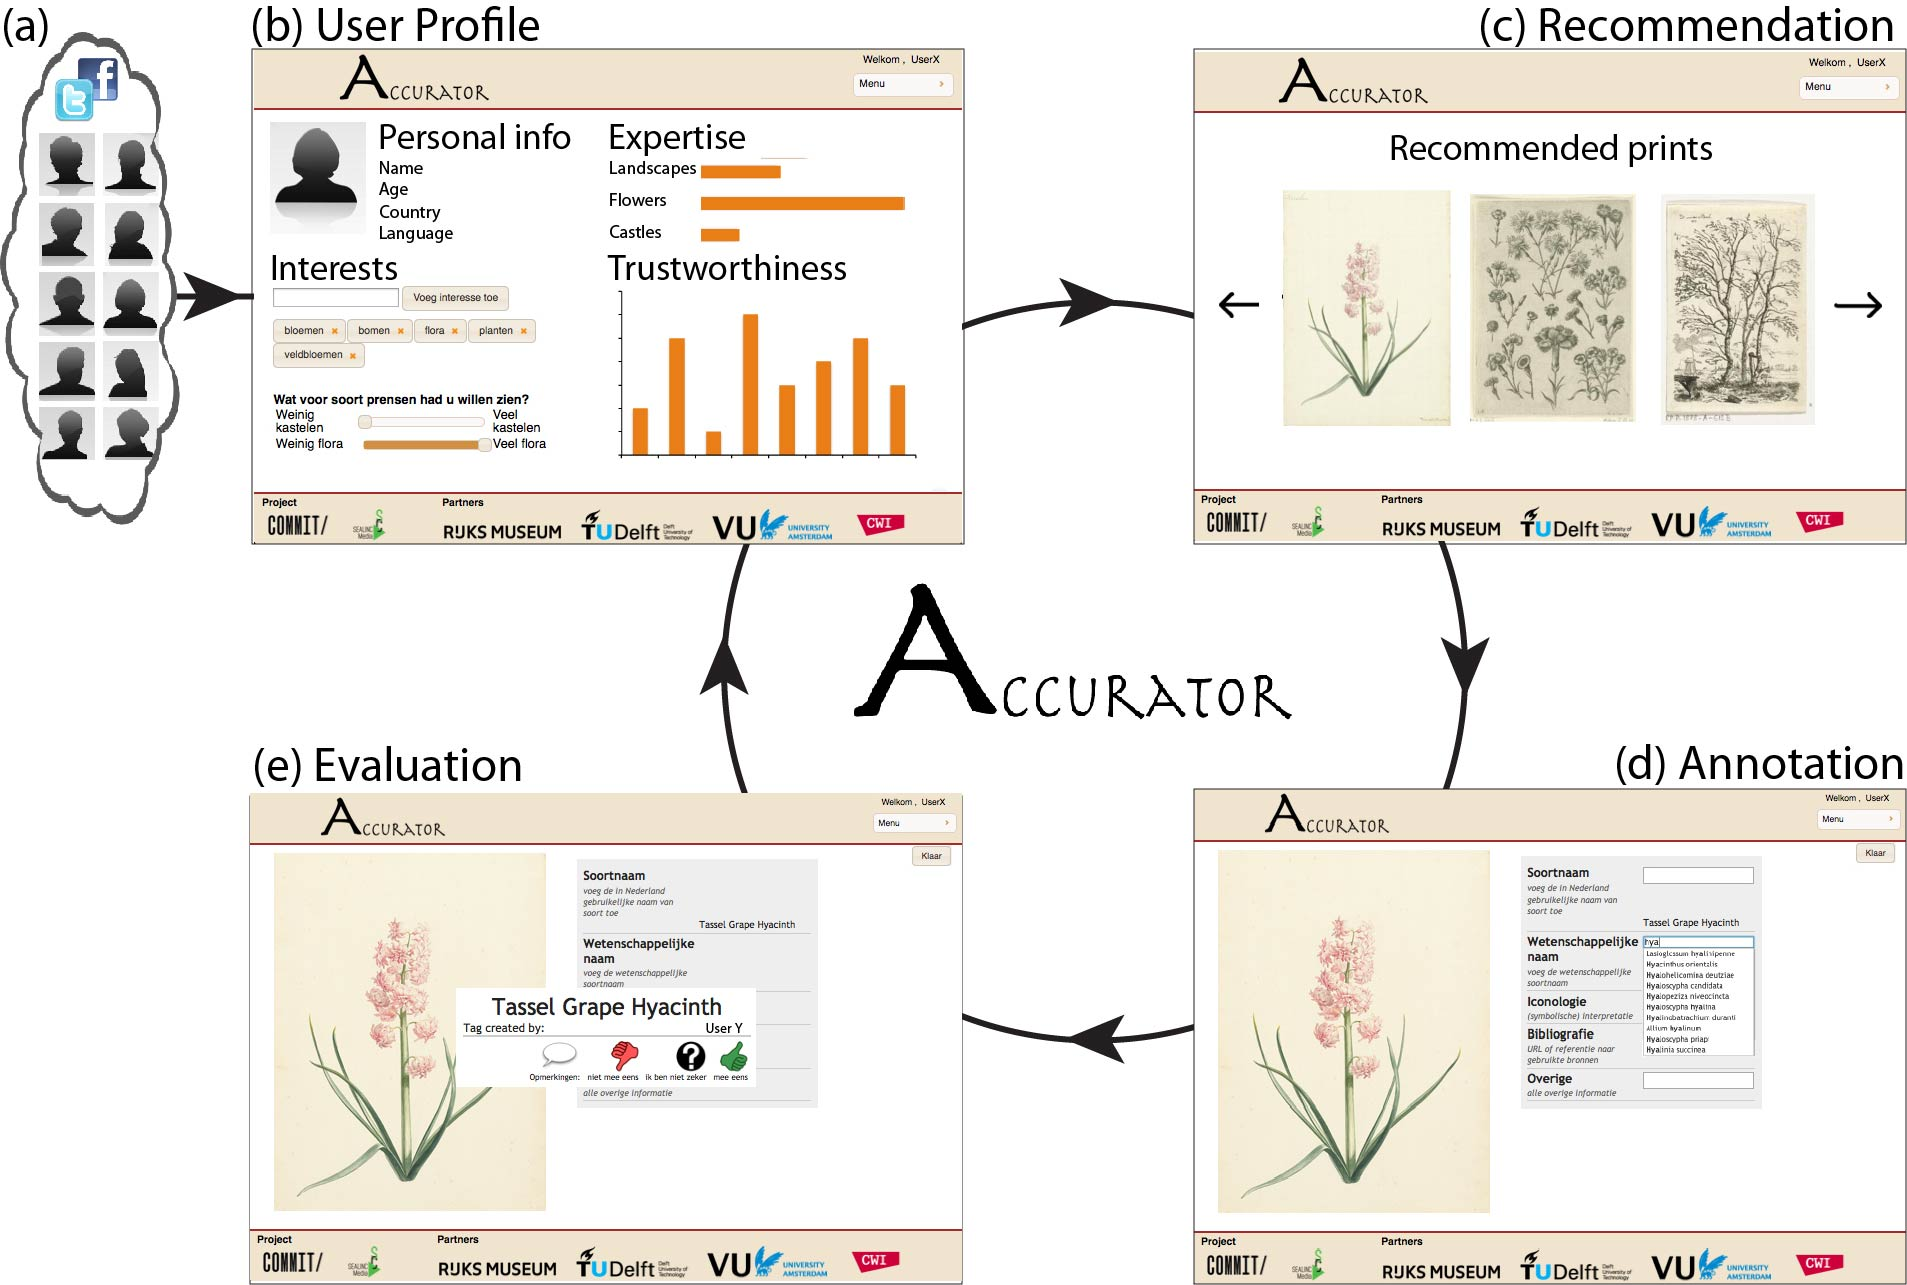
\includegraphics[width=\textwidth]{accurator_diagram.jpg}
  	\caption{Accurator personalized nichesourcing workflow}
\end{figure*}

The process starts (see Figure 1a) with searching the social web for user generated content that is relevant for a specific topic. We calculate the relevance of the content creators with respect to the topic and exploit social relations to identify a topical niche. When a person starts using Accurator, a user profile (see Figure 1b) is build based on available data.
% and shown to the user. The user can specify additional social web accounts.

Figure 1c shows the recommendation of collection items for a user. The recommendation strategy is based on specific patterns in the data, the user profile and the current annotation quality of an item. Accurator allows to easily change between different strategies to cater for users diversity.
% and a future task is to automatically adapt the choice of strategy based on that user profile. 
The choice of recommended item will affects the calculated interest of that user.

Figure 1d shows the interface where users add their annotations to an item. The presented fields dependent on the topic and the user's expertise on that topic. 
%Users with more expertise on that topic are allowed to enter more difficult fields. 
Accurator can also be configured to use domain vocabularies to support the user. Figure 1e shows the interface in which users can evaluate the annotations of other users. This task is only available to users who are trustworthy and have a certain level of expertise. The result of a review affects 1) the quality of an annotation, 2) the expertise level of the user and 3) the trustworthiness of another user.

% Another aspect that holds for all interfaces is that they should be intuitive and helpful. Users who encounter difficulties with the interface will not return. 

Accurator is build using Cliopatria to store RDF, GWT for the user interface and GAE for hosting. Accurator is now used for experimentation with data from the Rijksmuseum Amsterdam and a demo is available at \url{http://rma-accurator.appspot.com}.



